\documentclass{easychair}
\usepackage{authblk}
\usepackage{url}
\usepackage{paralist}

\begin{document}
\title{Using {\LaTeX} in Schools: Simplifying Inclusive STEM Education}

\author[1]{Barbara Henn\inst{1}\and Michael Schäffler\inst{1}\and Davide Cervone\inst{2} \and Volker Sorge\inst{2}\and
  Dorine in't Veld\inst{3}}
% \email{austind@gvsu.edu}
\institute{%
  SBBZ Ilvesheim, Germany
  \and
  MathJax Consortium
  \and
  Dedicon, The Netherlands
}

\titlerunning{Using {\LaTeX} in Schools: Simplifying Inclusive STEM Education}
\authorrunning{Henn, Schäffler, Cervone, Sorge, in't Veld}
\maketitle


\section{Introduction}\label{sec:intro}

We report on experience of the use of {\LaTeX} in Schools to teach mathematics
to blind and visually impaired children. For the last 20 years the German
education has phased out the use of sophisticated mathematical Braille notations
and replace it by teaching children from year one {\LaTeX} (or {\LaTeX}-like)
notation in mathematics. This notation made tactile by translating it into 8-dot
Euro Braille thus removing the use of indicators and the need to express single
characters with multiple Braille cells. The aim was to reduce the learning curve
for students as well as to improve their abilities to author and communicate
mathematics with peers and teachers that are not trained in Braille, which is
paramount for inclusive education.

There has been previous work on using {\LaTeX} as the basis for assistive
technologies, such as text-to-speech (TTS) translation~\cite{raman1994aster} or
for transcriptions of Braille textbooks~\cite{murillo2016latex}. These works
would transform {\LaTeX} into dedicated math speech systems or specialist math
Braille dialects like Marburg or Nemeth, rather then using the power of {\LaTeX}
directly and making it available as a communication medium for blind and
visually impaired (BVI) learners. We present how our approach can technically be
supported via web technology that can not only render {\LaTeX}, but also provide
8-dot Braille output for expressions as well as compute meaningful {\LaTeX}
commands for sub-expression and support for direct copying from web sites.

Finally, we will discuss our initial ideas to transfer this model to other
education systems, namely the Dutch system, where the current approach is
ambivalent, in that there exists an AsciiMath-like linearized math notation for
teaching to BVI students, while tactile math textbooks use an outdated Braille
notation, that is effectively no longer used in teaching.  As a result, students
are actively discouraged from studying mathematics.

\section{{\LaTeX} in Education for the Blind}\label{sec:latex-in-schools}

The choice of mathematical notation in education for blind and visually impaired
(BVI) students vary widely throughout the world. While there exist many national
and regional variations in regular mathematical notation, these differences are
particularly strong for primary and secondary education and become less
pronounced in advanced mathematics and higher education. For BVI learners
however this is generally not the case.

Traditionally, mathematics is presented in tactile format on the basis of highly
specialized Braille notations, which increases in complexity for more advanced
mathematical notation and more unconventional symbols. In particular, in
traditional 6-dot Braille systems symbols have to be embellished with a plethora
of indicators (e.g., for numbers, capital letter, fonts) and modifiers (for
accents, positioning etc.). For a comparison of notational systems
see~\cite{van2022towards}.

This approach has a number of drawbacks: 
\begin{inparaenum}[(1)]
\item The learning curve for mathematics, already steep for sighted students,
  becomes even steeper for BVI students.
\item Students can not easily communicate their Braille math with their sighted
  peers or teachers not trained in the formalism, which is an obstacle for
  inclusive education.
\item Math Braille notation is usually easier to read but less suitable for
  writing mathematics. This is particularly compounded by the use of computers
  even with Braille input devices.
\item Many traditional Math Braille notations have a 2D variant for complex
  elements like nested fractions or matrices, which are difficult to display on
  a computer Braille display.
\item Different Math Braille notations are generally not compatible and often
  even mutually intelligible. Not only have different countries different
  notations, but even the same language has different Math Braille dialects,
  e.g., in English there exist Nemath and UEB as well as formerly British Math
  Braille etc.
\end{inparaenum}


As a consequence more than 20 years ago Germany has chosen a different path for
specialist education for BVI students~\cite{kalina93, kalina98, Lorenz02},
replacing the teaching of the local mathematical Braille notation (Marburg
System) based on 6-dot Braille by adopting a uniform {\LaTeX} notation for writing
and transcribing that notation into 8-dot Euro Braille.

Since the early 1990s, the number of blind students in mainstream schools in
Germany rose significantly. This increase was mainly due to the technical
developments, with students working consistently with a PC and a connected
Braille display, using 8-dot Braille, as opposed to the traditional six
dots. Employing 8-dot font did not only prove less difficult for use with a
computer, but also advantageous for inclusive education, as it turned out that
8-dot Braille was more compatible with the world of the sighted classmates.

For every character, letter, and number that had to be learned by the sighted
student, there was exactly one equivalent in 8-dot Braille. There was no need
for duplicate meanings of characters or indicators and modifiers as every single
ASCII character can be translated into its equivalent Euro Braille cell.
  
Consequently, in the 2000s, a debate broke out in Germany between the competing
writing systems of 6-dot and 8-dot Braille. While 6-dot script with and without
contraction were mainly used in schools for the blind, the 8-dot script was the
Braille system for integrated education and inclusion~\cite{hallmann01}.  This
long-standing practice was scientifically underpinned by the Zubra study conducted
by Lang et al~\cite{Lang20, Zubra}, which demonstrated that sufficient reading
speed is also possible with 8-dot Braille. Moreover, in combination with screen
reader output, reading speed is much higher than reading contracted 6-dot
Braille on paper.

In mathematical writing the script that goes hand in hand with 8-dot Braille is
the {\LaTeX} typesetting system as every single character of the {\LaTeX} code
corresponds to exactly one Braille cell. In elementary school mathematics,
{\LaTeX} code is only necessary in a few places, as the digits and arithmetic
symbols are already available in the 8-dot system. However, some characters,
such as the element symbol, are introduced in {\LaTeX} notation.  With the
transition to secondary school, the {\LaTeX} commands for fractions, root signs
and exponent notation are added. Thus, on the way to the secondary school
examination (Abitur), the students are gradually taught all the necessary
{\LaTeX}.

For teachers in mainstream schools, {\LaTeX} is not a major hurdle, as many
mathematics teachers are already familiar with this system from
University. Those who are new to it can quickly learn it due to its intuitive
and semantic notation.  In contrast, both 6-dot contracted Braille and the 6-dot
mathematical notation in Germany --- the Marburg system --- are much more
complex to learn. As a result, learning these notations is hardly feasible
for teachers in mainstream schools. The 8-dot Braille system, together with the
linear notation of {\LaTeX} on the one hand and the PC in conjunction with a
screen reader and a Braille display on the other, represent an ideal bridging
technology between the sighted and blind worlds. {\LaTeX} not only helps
students to communicate mathematics with their teachers but also with their
sighted peers. Simple expressions are easy to understand even for those not yet
exposed to {\LaTeX} syntax. And if that fails it can be visually rendered for
easier reading.

With the increasing digitalization in schools for blind students and the
introduction of computers in every classroom, the 8-dot system and {\LaTeX} have
become the widely accepted standard. Many students thus achieve the University
entrance qualification and can continue to work seamlessly at Universities with
{\LaTeX}~\cite{bexten2002latex}. As {\LaTeX} is the lingua franca among
mathematicians and as such internationally understood notation, students going
on to higher education are already equipped with the most important tool to
communicate mathematics with their professors.


\section{{\LaTeX} to Braille}\label{sec:latex-to-Braille}

As already mentioned, in early primary education very little {\LaTeX} is actually
needed. And even then the main goal is to use as much as possible symbols that
are available on the keyboard. For example, asterisk \texttt{*} is used instead
of \verb+\cdot+ for multiplication and simple fractions are written in beveled
notation e.g., $\frac{1}{2}$ would be written as \texttt{1/2} instead of
\verb+\frac{1}{2}+. Nevertheless, some symbols like $\in$ are already introduced
in their {\LaTeX} notation \verb+\in+.

Other conventions are adopted for easier reading, such as avoiding curly braces
as much as possible, and inserting spaces before operators and relation
symbols. Consider the example ${ n! = n*(n-1)! }$ that is written by
this convention as \verb+n! =n *(n -1)!+ In addition, certain command abbreviations
are introduced, primarily with the goal of reducing spatial requirements on the
Braille display. E.g., writing \verb+\f+ instead of \verb+\frac+, or \verb+\ol+
instead of \verb+\overline+ . Also commands can be replaced by meaningful symbol
combinations, such as \verb+\le+ being replaced by \verb+<=+ (see also
\url{https://augenbit.de/}).

Initial online support for working with {\LaTeX} and Euro Braille was developed
at the SBBZ Ilvesheim as an extension of the MathJax v2.7~\cite{MathJax16-w4a}
library. The extension allowed to expose the {\LaTeX} sources in the web page
from which the MathJax would compute the visual rendering as textual underlay
for the expression. This allowed easy selection and copying and pasting into a
text editor or word processor from which the expression could be automatically
translated into 8-dot Braille by a correctly configured screen reader. While
this technique was sufficient for students to work with, in particular during
the Covid pandemic, it had the drawback that, while some cleanup on the {\LaTeX}
source could be done, the expression would usually not follow all the rules
described above.

In MathJax version 4~\cite{mathjax20siam} we will support these features
natively, in particular, copying and Euro Braille translation and rewriting
{\LaTeX} sources into the required format. Figure~\ref{fig:euroBraille} shows
the Braille translation for the commands describing the quadratic equation:

\[
\verb+x = \frac{-b \pm \sqrt{b^2-4ac}}{2a}+
\]

\begin{figure}
  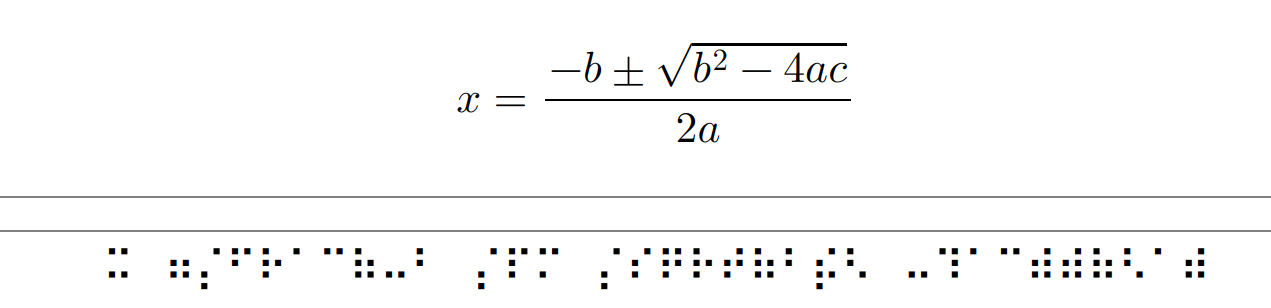
\includegraphics[width=.9\textwidth]{quadratic.png}
  \caption{Translation of the quadratic equation into 8-dot Euro Braille}
  \label{fig:euroBraille}
\end{figure}

As an additional feature MathJax v4 exposes correct {\LaTeX} sub expressions for
parts of formulas that can be interactively explored. While this sounds
straightforward, these sub expressions are non-trivial to compute. Firstly,
{\LaTeX} is a touring complete language, which requires a recursive stack
automaton for parsing and thus partial expressions are not as readily available
as in a simple LR-parser. Secondly, the exploration is based on a semantic model
that is computed using Speech Rule Engine~\cite{sre}, which produces a
canonical purely semantic representation of the math expression regardless of
the incoming syntax, i.e., {\LaTeX}, MathML, or AsciiMath..

\begin{figure}
  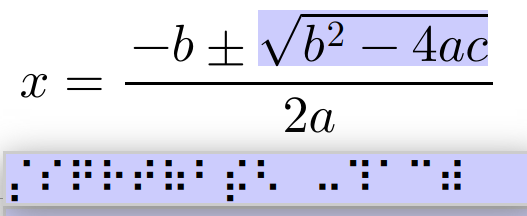
\includegraphics[width=.6\textwidth]{quadratic-square.png}
  \caption{Translation of the quadratic equation into 8-dot Euro Braille}
  \label{fig:subBraille}
\end{figure}

Figure~\ref{fig:subBraille} shows the Braille for the square root sub expression
in the quadratic formula.\footnote{Additional examples of the technique can be found
here: \url{https://mathjax.github.io/MathJax-demos-web/euro-Braille/}} Note that
there are nevertheless limits to the {\LaTeX} sub expression MathJax can
produce. For example, AMS matrix environments like \texttt{pmatrix},
\texttt{bmatrix}, or \texttt{vmatrix} implicitly generate fences, that are
rendered. However, at the moment the parsing algorithm cannot produce
corresponding {\LaTeX} output.

\section{Math Notation in the Netherlands}\label{sec:math-netherlands}

While similar approaches to Math Braille notation have been taken in other
European countries using established mathematical syntax notations (e.g.,
{\LaTeX} in Slovenia and AsciiMath in Sweden), other countries have pursued a
different approach.

We will examine the situation in The Netherlands. Over twenty years ago in The
Netherlands math had become practically inaccessible, the primary problem being
the lack of a Math Braille code. Consequently, a linear notation was developed
and introduced by Dedicon\footnote{\url{http://Braille.dedicon.nl/wiskunde}},
which eases math communication in particular in inclusive education, but did not
follow any pre-existing standards. In fact, the Dedicon notation is a mix of
several linear notations, borrowed from symbolic calculation languages, like
Maple, Mathematica, Excel. Pragmatic choices were made to make the notation as
intuitive as possible; e.g. using SQR, SQRT or the dutch word WORTEL for
abbreviations of square root.

In~\cite{Dorine16}, Dorine in‘t Veld and Davy Kager presented the status of this
notation, which in practice works quite well for students, since it meets all
the needs summed up above for {\LaTeX}:
\begin{enumerate}
\item It allows direct communication with sighted peers and teachers.
\item It remains consistent notwithstanding in what application it is used. It
  can be converted from Microsoft Word or HTML to plain text or Markdown without
  any problems, because, like {\LaTeX}, the notation only uses ASCII characters
  that can be typed with a qwerty keyboard.
\item It requires no additional assistive or conversion software. The
  screenreader translates the notation to 8-dot Braille and TTS.
\end{enumerate}


% One of the notation's strong points is that it remains consistent
% notwithstanding in what application it is used. It can be converted from
% Microsoft Word or HTML to plain text or Markdown without a problem. That is
% because the notation only uses characters that can be typed with a qwerty
% keyboard. It can be used for direct communication without requiring additional
% assistive or conversion software. Likewise, its translation into Braille is
% straightforward in particular when using 8-dot Euro Braille.

The weaknesses are that the notation initially only covered primary and
secondary education, not higher education. And while it was good for writing, it
was too ambiguous for more complex expressions, mainly due to its use of spaces
for delineation. For example, there is a rule that spaces terminate superscript
and subscript text, which is usually very convenient but can go wrong when
combining the two: Consider \verb+x_2 ^2+ versus \verb+x_2^2+, where the former
is $x_2^2$, while the latter represents $x_{2^2}$. Note that the space between the
$2$ and the caret symbol makes the difference, which can lead to easy mistakes.
The main issue is the lack of clear notation that defines argument boundaries,
which is particularly concerning with more complex expressions containing
fractions, roots, vectors etc.  As a consequence, automatic conversion is
difficult and there currently exists no implementation of a renderer that can
visualize expressions.

As already mentioned, the Dedicon notation is quite popular with students and
teachers in The Netherlands and it works sufficiently well in practice. And
since Dedicon has the responsibility to make textbooks accessible, they must use
formats that are actually taught to students, which currently means that books
are transcribed into Word documents with math in Dedicon notation.

As a consequence the necessary improvements indicated in 2016 have not been made
yet. Likewise there is no pressure to change to AsciiMath or {\LaTeX} for
schools or to extend the current Dedicon notation to become suitable for more
advanced mathematics.
However, this leads to a disconnect on the other stages of the education ladder:

\begin{enumerate}
\item Students in higher education have no support of specialized itinerant
  teachers who are experts in a discipline and in the use of screenreaders. This
  means for example that those students who need to learn {\LaTeX} at their
  University, have to find a practical accessible tutorial on their
  own. Additionally, if they do not have the luck to find someone in their
  IT-department who can help out, they have to find out what software to use and
  how it can be installed in the network of their University, etc.
\item Students in secondary pre academic education already have no support of
  specialized itinerant teachers. In fact they too are pretty much on their own
  with their laptop and screenreader. The last couple of years there is much
  more attention for science education; there is a working group that develops
  (mainly tactile) materials and there is a helpdesk. But there was no attention
  for standard mathematics notation like {\LaTeX} so far; there were many other
  priorities and – again – the Dedicon notation works well enough.
\end{enumerate}

This matter is compounded by another peculiar problem in primary schools:
children often want printed Braille, also for math. In these tactile books an
old 6-dot Braille math code is used, that is not taught to the students. When they
start from scratch they will easily learn and accept that spacing rules are
different in Braille and if there might be a notation they do not understand,
they can ask their teacher or peers what the original book says or they can look
up things in a symbols list. For secondary and higher education, we no longer
print Braille. The educational institutes for the BVI students do not want it
since the code for more advanced math is too complex and nobody learns it. For
tactile images this means, that it is often not possible to transcribe formulas
into Braille, if they cannot be expressed in 6-dot Braille.

Moreover math is mostly done electronically on the laptop in secondary
school. Until fairly recently students would choose their own preferred 8-dot
Braille table on their Braille display, mostly the ‘German’ or ‘American’
table. While students are now encouraged to mostly use Euro Braille, those who
are used to other Braille tables, are often reluctant to change to Euro
Braille.

Due to the fact that students are very much on their own finding their way and
there is no uniform notation or code, still only very few blind students choose
science studies where they need more advanced mathematical notation and
specialized software applications. Because of the same reasons, many students
experience big obstacles in disciplines that require statistics. Here R becomes
more prevallent with strong community support and improving accessibility
support based on {\LaTeX}. This, together with the advantages to be learned from
the German system, in combination with the latest MathJax developments, should
help to improve the situation in The Netherlands and bring about a feeling of
urgency to have books from which you can simply copy (human readable) {\LaTeX}
that one can communicate, render or paste into accessible software thereby
increasing the number of BVI students taking up mathematical and scientific
subjects in secondary and higher education. Hopefully this article will raise
awareness and involve experts from the above mentioned working group to push
this agenda forward.


% As an initial step we therefore aimed at moving from the Dedicon notation to
% AsciiMath. However, we are now in the process of exploring the possibility to
% follow the German model and introducing {\LaTeX} as the basic language of math
% exchange.  One major obstacle that we need to overcome is that our current
% production pipeline for electronic documents, translates printed math material
% into MathML rather than into {\LaTeX}, which would be more future proof and more
% helpful for the students in the next generations.

% \clearpage
\bibliographystyle{plain}
\bibliography{bibs}


\end{document}


%%% Local Variables:
%%% mode: latex
%%% TeX-master: t
%%% End:
